% ==============================================================================
% BÁO CÁO BÀI TẬP LỚN KẾT THÚC MÔN KHAI PHÁ DỮ LIỆU
% Đề tài: Nghiên cứu và cải tiến thuật toán BFSPMiner
% Format: Bài tập lớn Thạc sĩ (report class)
% ==============================================================================
\documentclass[14pt,a4paper,oneside]{extreport}

% --- PACKAGES ---
\usepackage[utf8]{inputenc}
\usepackage[vietnamese]{babel}
\usepackage{vntex}
\usepackage{mathptmx} % Times New Roman
\usepackage{amsmath,amssymb,amsfonts}
\usepackage{graphicx}
\usepackage{booktabs}
\usepackage{multirow}
\usepackage{longtable}
\usepackage{array}
\usepackage{tabularx}
\usepackage{algorithm}
\usepackage{algorithmic}
\usepackage{listings}
\usepackage{xcolor}
\usepackage{hyperref}
\usepackage{caption}
\usepackage{subcaption}
\usepackage[numbers,sort&compress]{natbib} % Trích dẫn dạng số [1,2,3]
\usepackage{geometry}
\usepackage{fancyhdr}
\usepackage{setspace}
\usepackage{indentfirst}
\usepackage{titlesec}
\usepackage{etoolbox}
\AtBeginEnvironment{algorithm}{\onehalfspacing}
\usepackage{tikz}
\usetikzlibrary{trees,arrows.meta,positioning,shapes}
\usepackage{float}
% --- LIST FORMATTING ---
\usepackage{enumitem}
\setlist{leftmargin=0pt, labelindent=1.0cm, labelwidth=0pt, labelsep=0.8em, itemindent=!, align=left, itemsep=0pt, parsep=0pt, topsep=0pt, partopsep=0pt}

% --- BIBLIOGRAPHY FORMATTING ---
\makeatletter
\renewenvironment{thebibliography}[1]
     {\chapter*{\bibname}%
      \addcontentsline{toc}{chapter}{\bibname}%
      \list{\@biblabel{\@arabic\c@enumiv}}%
           {\settowidth\labelwidth{\@biblabel{9}}%
            \leftmargin 0pt
            \labelsep 0.5em
            \itemindent \dimexpr \labelwidth + \labelsep \relax
            \itemsep 0pt
            \parsep 0pt
            \let\makelabel\bibmakelabel
            \usecounter{enumiv}%
            \let\p@enumiv\@empty
            \renewcommand\theenumiv{\@arabic\c@enumiv}}%
      \sloppy
      \clubpenalty4000
      \@clubpenalty \clubpenalty
      \widowpenalty4000%
      \sfcode`\.\@m}
     {\def\@noitemerr
       {\@latex@warning{Empty `thebibliography' environment}}%
      \endlist}
\def\bibmakelabel#1{#1\hfill}
\makeatother

% --- TOC/LOF/LOT SPACING CONFIGURATION ---
\usepackage[titles]{tocloft}
\setlength{\cftbeforechapskip}{0pt}
\setlength{\cftbeforesecskip}{0pt}
\setlength{\cftbeforesubsecskip}{0pt}
\setlength{\cftbeforefigskip}{0pt}
\setlength{\cftbeforetabskip}{0pt}

\setlength{\cftchapindent}{0pt}
\setlength{\cftsecindent}{0pt}
\setlength{\cftsubsecindent}{0pt}
\setlength{\cftfigindent}{0pt}
\setlength{\cfttabindent}{0pt}

% --- PAGE SETUP ---
\geometry{
    top=3.5cm,
    bottom=3.0cm,
    left=3.5cm,
    right=2.0cm,
    headheight=17pt
}

% --- SPACING ---
\onehalfspacing
\setlength{\parskip}{0pt}
\setlength{\parindent}{1.0cm}
\raggedbottom

% --- HEADER/FOOTER ---
\pagestyle{fancy}
\fancyhf{}
\fancyhead[C]{\thepage} % Đánh số trang ở giữa phía trên
\renewcommand{\headrulewidth}{0pt} % Xóa đường kẻ ngang

% Ghi đè plain style (do \chapter tự động gọi) để số trang vẫn nằm ở trên cùng
\fancypagestyle{plain}{
    \fancyhf{}
    \fancyhead[C]{\thepage}
    \renewcommand{\headrulewidth}{0pt}
}

% --- CODE LISTING STYLE ---
\definecolor{codegreen}{rgb}{0,0.6,0}
\definecolor{codegray}{rgb}{0.5,0.5,0.5}
\definecolor{codepurple}{rgb}{0.58,0,0.82}
\definecolor{backcolour}{rgb}{0.97,0.97,0.97}

\lstdefinestyle{pythonstyle}{
    backgroundcolor=\color{backcolour},
    commentstyle=\color{codegreen},
    keywordstyle=\color{blue}\bfseries,
    numberstyle=\tiny\color{codegray},
    stringstyle=\color{codepurple},
    basicstyle=\ttfamily\footnotesize,
    breakatwhitespace=false,
    breaklines=true,
    captionpos=b,
    keepspaces=true,
    numbers=left,
    numbersep=5pt,
    showspaces=false,
    showstringspaces=false,
    showtabs=false,
    tabsize=2,
    frame=single,
    language=Python,
    extendedchars=false
}
\lstset{style=pythonstyle}

% --- CHAPTER TITLE FORMAT ---
\titleformat{\chapter}[block]
  {\normalfont\Large\bfseries\centering}
  {\chaptertitlename\ \thechapter. }{0pt}{\Large\MakeUppercase}
\titlespacing*{\chapter}{0pt}{-24pt}{0pt}

\titleformat{\section}
  {\normalfont\normalsize\bfseries}
  {\thesection}
  {1em}
  {\MakeUppercase}
\titlespacing*{\section}{0pt}{0pt}{0pt}

\titleformat{\subsection}
  {\normalfont\normalsize\bfseries}
  {\thesubsection}
  {1em}
  {}
\titlespacing*{\subsection}{1.0cm}{0pt}{0pt}

\titleformat{\subsubsection}
  {\normalfont\normalsize\bfseries\itshape}
  {\thesubsubsection}
  {1em}
  {}
\titlespacing*{\subsubsection}{1.0cm}{0pt}{0pt}

% --- FLOAT SPACING ---
\setlength{\intextsep}{0pt}
\setlength{\floatsep}{0pt}
\setlength{\textfloatsep}{0pt}
\setlength{\abovecaptionskip}{0pt}
\setlength{\belowcaptionskip}{0pt}
\renewcommand{\arraystretch}{1.2}

% --- CAPTION FORMAT ---
\captionsetup{
    font={normalsize, stretch=1.5},
    labelfont=bf,
    labelsep=period,
    skip=0pt
}

% TOC and Section numbering limits
\setcounter{tocdepth}{2}
\setcounter{secnumdepth}{3}
\captionsetup[table]{position=above}
\captionsetup[figure]{position=below}

% --- HYPERREF SETUP ---
\hypersetup{
    colorlinks=true,
    linkcolor=blue!70!black,
    citecolor=blue!60!black,
    urlcolor=blue!80!black,
}

% ==============================================================================
\begin{document}


% --- MỤC LỤC ---
\renewcommand{\contentsname}{MỤC LỤC}
\pagenumbering{roman} % Đánh số La Mã cho các trang đầu
\cleardoublepage
\addcontentsline{toc}{chapter}{MỤC LỤC}
\begin{spacing}{1}
\tableofcontents
\end{spacing}
\newpage

% --- DANH MỤC HÌNH ---
\renewcommand{\listfigurename}{DANH MỤC HÌNH VẼ}
\cleardoublepage
\addcontentsline{toc}{chapter}{DANH MỤC HÌNH VẼ}
\begin{spacing}{1}
\listoffigures
\end{spacing}
\newpage

% --- DANH MỤC BẢNG ---
\renewcommand{\listtablename}{DANH MỤC BẢNG BIỂU}
\cleardoublepage
\addcontentsline{toc}{chapter}{DANH MỤC BẢNG BIỂU}
\begin{spacing}{1}
\listoftables
\end{spacing}
\newpage

% --- DANH MỤC CÁC CHỮ VIẾT TẮT ---
\chapter*{DANH MỤC CÁC CHỮ VIẾT TẮT}
\addcontentsline{toc}{chapter}{DANH MỤC CÁC CHỮ VIẾT TẮT}
\begin{itemize}
    \item \textbf{BFSPMiner}: Batch-Free Sequential Pattern Miner
    \item \textbf{IoT}: Internet of Things (Internet vạn vật)
    \item \textbf{SPM}: Sequential Pattern Mining (Khai phá mẫu tuần tự)
\end{itemize}
\newpage

% ==============================================================================
% CHƯƠNG 1: GIỚI THIỆU
% ==============================================================================
\clearpage
\pagenumbering{arabic}
\setcounter{page}{1} % Đánh số 1 bắt đầu từ phần nội dung chính
\chapter{Giới thiệu}
\label{chap:intro}

\section{Đặt vấn đề}
Khai phá mẫu tuần tự (Sequential Pattern Mining -- SPM) trên luồng dữ liệu liên tục là một bài toán trọng tâm trong lĩnh vực khai phá dữ liệu hiện đại~\cite{fournier2017}. Trong bối cảnh Internet vạn vật (IoT), thương mại điện tử và hệ thống thông tin quy mô lớn, dữ liệu phát sinh liên tục dưới dạng \textit{luồng} (stream) --- một chuỗi vô hạn các sự kiện đến với tốc độ cao và phân bố thay đổi theo thời gian.

Các ứng dụng thực tế đòi hỏi khả năng khai phá mẫu tuần tự trực tuyến bao gồm:
\begin{itemize}
    \item \textbf{Giám sát IoT:} Phát hiện các chuỗi hành vi bất thường từ cảm biến (ví dụ: tín hiệu tiêu thụ điện năng bất thường trong nhà thông minh).
    \item \textbf{Phân tích hành vi web:} Khai phá các chuỗi tương tác của người dùng trên website (clickstream) để tối ưu trải nghiệm và hệ thống gợi ý.
    \item \textbf{An ninh mạng:} Phát hiện các chuỗi sự kiện tấn công trong log hệ thống.
    \item \textbf{Tin sinh học:} Phân tích chuỗi DNA, protein theo thời gian thực.
\end{itemize}

Luồng dữ liệu mang ba đặc trưng thách thức khiến các thuật toán khai phá truyền thống (PrefixSpan \cite{pei2001}, SPADE \cite{zaki2001}) không thể áp dụng trực tiếp:
\begin{enumerate}
    \item \textbf{Vô hạn và liên tục:} Không thể lưu toàn bộ dữ liệu vào bộ nhớ.
    \item \textbf{Tốc độ cao:} Mỗi sự kiện cần được xử lý ngay lập tức (single-pass).
    \item \textbf{Phân bố thay đổi:} Các mẫu hành vi có thể thay đổi theo thời gian (concept drift).
\end{enumerate}

\section{Hạn chế của các phương pháp hiện tại}
Phần lớn các thuật toán khai phá mẫu tuần tự trên luồng dữ liệu dựa trên mô hình xử lý theo lô (\textit{batch-based})~\cite{marascu2006, ho2005}, chia luồng vô hạn thành các khối có kích thước cố định rồi khai phá từng khối. Cách tiếp cận này tồn tại hai vấn đề:

\begin{enumerate}
    \item \textbf{Mất mẫu qua ranh giới lô:} Các chuỗi mẫu nằm xuyên suốt nhiều batch bị bỏ sót hoàn toàn, dẫn đến kết quả khai phá không đầy đủ.
    \item \textbf{Cắt tỉa cục bộ sai lầm:} Quyết định loại bỏ trong từng batch có thể xóa các mẫu có tần suất cao trên toàn cục nhưng xuất hiện rải rác ở các batch khác nhau.
\end{enumerate}

Thuật toán BFSPMiner (Batch-Free Sequential Pattern Miner), được đề xuất bởi Hassani et al.~\cite{hassani2019}, khắc phục các nhược điểm trên bằng khung khai phá \textit{batch-free} (không chia lô). Tuy nhiên, phiên bản gốc tồn tại hai hạn chế:
\begin{itemize}
    \item Tham số chiều dài mẫu tối đa (\texttt{maxPatternLength}) cố định.
    \item Chỉ hỗ trợ mẫu liên tiếp (consecutive), bỏ qua các phụ thuộc hành vi bị gián đoạn.
\end{itemize}

\section{Mục tiêu nghiên cứu}
Bài tập lớn này thực hiện ba mục tiêu chính:
\begin{enumerate}
    \item \textbf{Nghiên cứu và cài đặt} thuật toán BFSPMiner gốc bằng Python, tối ưu cấu trúc dữ liệu so với bản Java.
    \item \textbf{Đề xuất hai cải tiến:}
    \begin{itemize}
        \item \textit{Adaptive maxPatternLength:} Tự động điều chỉnh chiều dài mẫu tối đa dựa trên entropy luồng và áp lực bộ nhớ.
        \item \textit{Gap-Aware Episode Mining:} Mở rộng quá trình sinh mẫu để phát hiện các phụ thuộc hành vi không liên tiếp.
    \end{itemize}
    \item \textbf{Đánh giá thực nghiệm} trên hai tập dữ liệu thực tế: REDD (IoT, 458K sự kiện) và MSNBC (clickstream, 424K sự kiện).
\end{enumerate}

\section{Cấu trúc báo cáo}
Báo cáo được tổ chức thành 7 chương:
\begin{itemize}
    \item \textbf{Chương 1:} Giới thiệu bài toán, mục tiêu nghiên cứu.
    \item \textbf{Chương 2:} Cơ sở lý thuyết, phát biểu bài toán, dữ liệu đầu vào/đầu ra.
    \item \textbf{Chương 3:} Thuật toán BFSPMiner gốc với minh họa chi tiết từng bước.
    \item \textbf{Chương 4:} Các cải tiến đề xuất (Adaptive + Gap-Aware).
    \item \textbf{Chương 5:} Thực nghiệm và kết quả.
    \item \textbf{Chương 6:} Hướng dẫn cài đặt và sử dụng chương trình.
    \item \textbf{Chương 7:} Kết luận và hướng phát triển.
\end{itemize}

% ==============================================================================
% CHƯƠNG 2: CƠ SỞ LÝ THUYẾT VÀ PHÁT BIỂU BÀI TOÁN
% ==============================================================================
\chapter{Cơ sở lý thuyết và phát biểu bài toán}
\label{chap:theory}

\section{Các khái niệm cơ bản}

\subsection{Luồng dữ liệu}
\textbf{Định nghĩa 2.1 (Luồng dữ liệu).} Một luồng dữ liệu (data stream) $S = \langle s_1, s_2, s_3, \dots \rangle$ là một chuỗi vô hạn các phần tử (item) $s_i \in \Sigma$, trong đó $\Sigma$ là bảng ký hiệu (alphabet) hữu hạn và mỗi $s_i$ đến tại thời điểm $t_i$ theo thứ tự tăng dần.

\textit{Ví dụ:} Trong hệ thống giám sát năng lượng, $\Sigma = \{$\texttt{fridge}, \texttt{light}, \texttt{washer}, \texttt{microwave}, \texttt{dishwasher}$\}$ và luồng $S = \langle$\texttt{fridge}, \texttt{light}, \texttt{fridge}, \texttt{washer}, \texttt{light}, $\dots\rangle$ ghi lại thứ tự các thiết bị tiêu thụ điện.

\subsection{Mẫu tuần tự}
\textbf{Định nghĩa 2.2 (Mẫu tuần tự liên tiếp).} Một mẫu tuần tự (sequential pattern) $p = \langle p_1, p_2, \dots, p_k \rangle$ là một chuỗi con liên tiếp (consecutive subsequence) của $S$ nếu tồn tại vị trí $i$ sao cho $s_i = p_1, s_{i+1} = p_2, \dots, s_{i+k-1} = p_k$.

\textit{Ví dụ:} Với $S = \langle a, b, a, b, c, d \rangle$, mẫu $\langle a, b, c \rangle$ là mẫu tuần tự liên tiếp (xuất hiện tại vị trí $i = 3$), nhưng $\langle a, c \rangle$ \textit{không phải} mẫu liên tiếp (vì $a$ và $c$ không kề nhau).

\subsection{Độ hỗ trợ, độ tin cậy và độ nâng}

\textbf{Định nghĩa 2.3 (Độ hỗ trợ -- Support).} Cho luồng $S$ đã quan sát $n$ phần tử. Độ hỗ trợ của mẫu $p$ là:
\begin{equation}
    \text{supp}(p) = \frac{\text{count}(p)}{n}
\end{equation}
trong đó $\text{count}(p)$ là số lần $p$ xuất hiện liên tiếp trong $n$ phần tử đầu tiên của $S$.

\textbf{Định nghĩa 2.4 (Mẫu phổ biến -- Frequent Pattern).} Mẫu $p$ được gọi là phổ biến nếu $\text{supp}(p) \geq \sigma$, với $\sigma$ là ngưỡng support tối thiểu do người dùng định nghĩa.

\textbf{Định nghĩa 2.5 (Độ tin cậy -- Confidence).} Với mẫu $p = \langle p_1, \dots, p_{k-1}, p_k \rangle$, confidence được định nghĩa:
\begin{equation}
    \text{conf}(p) = \frac{\text{count}(p)}{\text{count}(\langle p_1, \dots, p_{k-1} \rangle)}
\end{equation}
thể hiện xác suất $p_k$ xuất hiện ngay sau tiền tố $\langle p_1, \dots, p_{k-1} \rangle$.

\textbf{Định nghĩa 2.6 (Độ nâng -- Lift).} Lift đo mức độ tương quan giữa tiền tố và hậu tố:
\begin{equation}
    \text{lift}(p) = \frac{\text{supp}(p)}{\text{supp}(\langle p_1, \dots, p_{k-1} \rangle) \times \text{supp}(\langle p_k \rangle)}
\end{equation}
Lift $> 1$ cho thấy sự xuất hiện cùng nhau mang tính tích cực; Lift $= 1$ là độc lập; Lift $< 1$ là tiêu cực.

\subsection{Cây Inverted $T_0$}

\textbf{Định nghĩa 2.7 (Cây Inverted $T_0$).} Cây Inverted $T_0$ là một cây tiền tố (trie) lưu trữ các mẫu tuần tự theo thứ tự \textit{đảo ngược thời gian} --- sự kiện gần nhất nằm ở cấp gốc (root), sự kiện xa nhất ở cấp lá (leaf). Mỗi nút chứa:
\begin{itemize}
    \item \texttt{value}: ký hiệu item.
    \item \texttt{count}: số lần xuất hiện tích lũy.
    \item \texttt{batch\_count}: số batch mà nút đã xuất hiện.
    \item \texttt{tid}: batch ID tại thời điểm nút được tạo.
    \item \texttt{time\_stamps}: danh sách thời điểm xuất hiện gần nhất.
    \item \texttt{children}: bảng băm (HashMap) ánh xạ ký hiệu $\rightarrow$ nút con.
\end{itemize}

\textit{Lợi thế:} Việc lưu theo thứ tự đảo ngược giúp tra cứu ngữ cảnh (context lookup) hiệu quả --- khi dự đoán item tiếp theo, ta bắt đầu từ sự kiện gần nhất (root level) và duyệt xuống.

\section{Phát biểu bài toán}
\label{sec:problem}


\textbf{Bài toán (Khai phá mẫu tuần tự batch-free trên luồng dữ liệu):}

\textit{Cho:}
\begin{itemize}
    \item Một luồng dữ liệu vô hạn $S = \langle s_1, s_2, \dots \rangle$ với $s_i \in \Sigma$.
    \item Ngưỡng support tối thiểu $\sigma > 0$.
    \item Chiều dài mẫu tối đa $L_{max}$.
    \item Tham số cắt tỉa: $\alpha$, $\varepsilon$, $\delta$.
\end{itemize}

\textit{Yêu cầu:}
\begin{itemize}
    \item Phát hiện \textbf{liên tục} (online) tất cả các mẫu tuần tự phổ biến $p$ (với $|p| \leq L_{max}$ và $\text{supp}(p) \geq \sigma$).
    \item Quét dữ liệu \textbf{một lượt} (single-pass): mỗi item chỉ được đọc đúng một lần.
    \item Kiểm soát bộ nhớ ở mức hằng số thông qua cắt tỉa định kỳ.
    \item Hỗ trợ dự đoán item tiếp theo dựa trên các mẫu đã khai phá.
\end{itemize}


\section{Dữ liệu đầu vào và đầu ra}
\label{sec:io}

Để minh họa rõ ràng bài toán, chúng tôi trình bày ví dụ cụ thể với dữ liệu đầu vào và đầu ra tương ứng.

\subsection{Đầu vào}

\begin{table}[H]
    \centering
    \caption{Dữ liệu đầu vào minh họa}
    \label{tab:input}
    \begin{tabular}{ll}
        \toprule
        \textbf{Thành phần} & \textbf{Giá trị} \\
        \midrule
        Luồng sự kiện $S$ & $\langle a, b, a, b, c, a, b, a, b, c, d, a \rangle$ \\
        Số phần tử & $n = 12$ \\
        Bảng ký hiệu $\Sigma$ & $\{a, b, c, d\}$ \\
        \texttt{maxPatternLength} $L_{max}$ & $5$ \\
        Ngưỡng support $\sigma$ & $0.15$ \\
        \texttt{batchLength} & $6$ \\
        \texttt{delta} $\delta$ & $1000$ \\
        \bottomrule
    \end{tabular}
\end{table}

\subsection{Đầu ra}

\begin{table}[H]
    \centering
    \caption{Đầu ra: Tập mẫu tuần tự phổ biến}
    \label{tab:output}
    \begin{tabular}{clcccc}
        \toprule
        \textbf{STT} & \textbf{Mẫu (Pattern)} & \textbf{Count} & \textbf{Support} & \textbf{Confidence} & \textbf{Loại} \\
        \midrule
        1 & $(a)$        & 4 & 0.333 & ---   & unigram \\
        2 & $(b)$        & 4 & 0.333 & ---   & unigram \\
        3 & $(a, b)$     & 4 & 0.333 & 1.000 & bigram \\
        4 & $(c)$        & 2 & 0.167 & ---   & unigram \\
        5 & $(b, c)$     & 2 & 0.167 & 0.500 & bigram \\
        6 & $(a, b, c)$  & 2 & 0.167 & 0.500 & trigram \\
        \bottomrule
    \end{tabular}
\end{table}

\textbf{Dự đoán:} Với ngữ cảnh hiện tại là hai sự kiện gần nhất $\langle \dots, a \rangle$, hệ thống dự đoán top-3 item tiếp theo là: $[\texttt{c}, \texttt{d}, \texttt{a}]$.

\textbf{Giải thích:} Mẫu $(a, b)$ có support 0.333 và confidence 1.0, nghĩa là mỗi lần sự kiện $a$ xuất hiện, sự kiện $b$ \textit{luôn} theo sau. Mẫu $(a, b, c)$ có support 0.167, nghĩa là chuỗi $a \rightarrow b \rightarrow c$ xuất hiện 2/12 = 16.7\% thời gian.

\section{Tổng quan các thuật toán liên quan}

\begin{table}[H]
    \centering
    \caption{So sánh các thuật toán khai phá mẫu tuần tự}
    \label{tab:related}
    \begin{tabular}{lcccc}
        \toprule
        \textbf{Thuật toán} & \textbf{Loại} & \textbf{Batch-free} & \textbf{Gap} & \textbf{Adaptive} \\
        \midrule
        PrefixSpan \cite{pei2001}  & Tĩnh    & Không & Không & Không \\
        SPADE \cite{zaki2001}      & Tĩnh    & Không & Có    & Không \\
        GSP \cite{srikant1996}     & Tĩnh    & Không & Có    & Không \\
        Batch-based SPM            & Luồng   & Không & Không & Không \\
        BFSPMiner \cite{hassani2019} & Luồng & \textbf{Có} & Không & Không \\
        \textbf{BFSPMiner-Improved} & Luồng & \textbf{Có} & \textbf{Có} & \textbf{Có} \\
        \bottomrule
    \end{tabular}
\end{table}

% ==============================================================================
% CHƯƠNG 3: THUẬT TOÁN BFSPMINER GỐC
% ==============================================================================
\chapter{Thuật toán BFSPMiner gốc}
\label{chap:algorithm}

Chương này trình bày chi tiết thuật toán BFSPMiner (Batch-Free Sequential Pattern Miner) được đề xuất bởi Hassani et al. \cite{hassani2019}, bao gồm kiến trúc tổng quan, các bước xử lý chính, và minh họa từng bước trên dữ liệu cụ thể.

\section{Tổng quan kiến trúc}

BFSPMiner xử lý luồng dữ liệu theo mô hình \textit{one-pass} (một lượt) với pipeline gồm 4 bước chính cho mỗi sự kiện đến:

\begin{enumerate}
    \item \textbf{Nhận sự kiện:} Đọc item mới từ luồng.
    \item \textbf{Sinh mẫu và cập nhật cây:} Xây dựng danh sách mẫu đảo ngược, chèn vào cây Inverted $T_0$.
    \item \textbf{Theo dõi lô:} Đếm số item đã xử lý để xác định ranh giới batch logic.
    \item \textbf{Cắt tỉa SSBE:} Định kỳ loại bỏ các nút không triển vọng khỏi cây.
\end{enumerate}

Sau khi xử lý toàn bộ luồng (hoặc tại bất kỳ thời điểm nào), có thể thực hiện:
\begin{itemize}
    \item \textbf{Trích xuất mẫu phổ biến:} Duyệt DFS cây, thu thập các mẫu có support $\geq \sigma$.
    \item \textbf{Dự đoán item tiếp theo:} So khớp ngữ cảnh gần nhất với các mẫu, xếp hạng theo confidence.
\end{itemize}

\section{Bước 1: Xây dựng cây Inverted $T_0$}
\label{sec:build_tree}

Khi nhận sự kiện mới $s_t$ tại thời điểm $t$, thuật toán thực hiện:

\begin{enumerate}
    \item Thêm $s_t$ vào danh sách sự kiện: $\textit{events}.\text{append}(s_t)$.
    \item Xây dựng danh sách mẫu đảo ngược (reversed pattern list):
    \begin{equation}
        \textit{pattern\_list} = [s_t, s_{t-1}, s_{t-2}, \dots, s_{t-L_{max}+1}]
    \end{equation}
    (lấy tối đa $L_{max}$ phần tử gần nhất theo thứ tự đảo ngược).
    \item Duyệt \textit{pattern\_list} từ trái sang phải, tại mỗi bước:
    \begin{itemize}
        \item Nếu nút con tương ứng \textbf{đã tồn tại}: tăng \texttt{count} lên 1.
        \item Nếu nút con \textbf{chưa tồn tại}: tạo nút mới với \texttt{count} = 1.
    \end{itemize}
\end{enumerate}

\begin{algorithm}[!ht]
\small
\caption{Thêm sự kiện vào cây Inverted $T_0$}
\label{alg:add_event}
\begin{algorithmic}[1]
\REQUIRE Cây $\mathcal{T}$, sự kiện $s_t$, batch hiện tại $b$
\STATE $\mathcal{T}.\textit{events}.\text{append}(s_t)$
\STATE $t \leftarrow |\mathcal{T}.\textit{events}| - 1$
\STATE $\textit{pattern\_list} \leftarrow [s_{t-i} \mid i = 0, 1, \dots, \min(L_{max}, t+1) - 1]$
\STATE $\textit{visited} \leftarrow \emptyset$ \COMMENT{Tránh đếm trùng}
\STATE $\textit{node} \leftarrow \mathcal{T}.\textit{root}$
\FOR{$i = 0$ \TO $|\textit{pattern\_list}| - 1$}
    \STATE $\textit{item} \leftarrow \textit{pattern\_list}[i]$
    \IF{$\textit{item} \in \textit{node}.\textit{children}$}
        \STATE $\textit{node} \leftarrow \textit{node}.\textit{children}[\textit{item}]$
        \IF{$\text{id}(\textit{node}) \notin \textit{visited}$}
            \STATE $\textit{node}.\textit{count} \leftarrow \textit{node}.\textit{count} + 1$
            \STATE $\textit{visited}.\text{add}(\text{id}(\textit{node}))$
        \ENDIF
    \ELSE
        \STATE $\textit{new\_node} \leftarrow \text{TreeObject}(\textit{item}, \textit{node}, b)$
        \STATE $\textit{node}.\textit{children}[\textit{item}] \leftarrow \textit{new\_node}$
        \STATE $\textit{node} \leftarrow \textit{new\_node}$
        \STATE $\textit{visited}.\text{add}(\text{id}(\textit{node}))$
    \ENDIF
\ENDFOR
\STATE $\mathcal{T}.\textit{root}.\textit{count} \leftarrow |\mathcal{T}.\textit{events}|$
\end{algorithmic}
\end{algorithm}
\vspace{-0.5em}

\section{Bước 2: Cắt tỉa SSBE}
\label{sec:ssbe}

Để kiểm soát kích thước cây, BFSPMiner sử dụng chiến lược cắt tỉa SSBE (Single-Scan Batch Error). Cứ sau mỗi $\delta$ batch, thuật toán duyệt đệ quy từng nút và kiểm tra điều kiện loại bỏ an toàn:

\begin{equation}
    c.\textit{count} + b' \times (\lceil \alpha \times l \rceil - 1) \leq \varepsilon \times b_s \times l
\end{equation}

trong đó:
\begin{itemize}
    \item $c.\textit{count}$: tần suất tích lũy của nút $c$.
    \item $b_s$: số batch kể từ khi nút $c$ được tạo.
    \item $b'$: số batch mà $c$ vắng mặt ($b' = b_s - c.\textit{batch\_count}$).
    \item $\alpha$: tỷ lệ tăng tối đa mỗi batch (mặc định 0.05).
    \item $\varepsilon$: ngưỡng pruning (mặc định 0.1).
    \item $l$: chiều dài luồng hiện tại.
\end{itemize}

\textbf{Ý nghĩa:} Ngay cả trong kịch bản \textit{lạc quan nhất} (giả sử nút xuất hiện tối đa $\lceil \alpha \times l \rceil - 1$ lần trong mỗi batch bị thiếu), nếu tần suất vẫn không vượt ngưỡng, nút đó chắc chắn không bao giờ trở thành mẫu phổ biến và được loại bỏ an toàn.

\begin{algorithm}[!ht]
\small
\caption{Cắt tỉa SSBE}
\label{alg:ssbe}
\begin{algorithmic}[1]
\REQUIRE Nút $n$, batch hiện tại $b$, tham số $\alpha$, $\varepsilon$, $\delta$, chiều dài luồng $l$
\FOR{mỗi nút con $c$ của $n$}
    \STATE $b_s \leftarrow b - (c.\textit{tid} - c.\textit{tid} \bmod \delta)$ \COMMENT{Số batch kể từ lần tạo}
    \STATE $b' \leftarrow b_s - c.\textit{batch\_count}$ \COMMENT{Số batch vắng mặt}
    \IF{$c.\textit{count} + b' \times (\lceil \alpha \times l \rceil - 1) \leq \varepsilon \times b_s \times l$}
        \STATE Xóa $c$ và toàn bộ cây con \COMMENT{Loại bỏ an toàn}
    \ELSE
        \STATE \textsc{SSBEPrune}($c, b, \alpha, \varepsilon, \delta, l$) \COMMENT{Đệ quy}
    \ENDIF
\ENDFOR
\end{algorithmic}
\end{algorithm}
\vspace{-0.5em}

\section{Bước 3: Trích xuất mẫu phổ biến}

Tại bất kỳ thời điểm nào, có thể trích xuất tập mẫu phổ biến bằng cách duyệt DFS (Depth-First Search) toàn bộ cây:

\begin{enumerate}
    \item Bắt đầu từ gốc, duyệt từng nhánh.
    \item Tại mỗi nút, tính $\text{supp} = \frac{c.\textit{count}}{\textit{root}.\textit{count}}$.
    \item Nếu $\text{supp} \geq \sigma$: thu thập đường đi từ gốc đến nút, \textbf{đảo ngược} lại để được mẫu gốc.
    \item Tính confidence = $\frac{c.\textit{count}}{\textit{parent}.\textit{count}}$.
\end{enumerate}

\textbf{Lưu ý quan trọng:} Vì cây lưu theo thứ tự đảo ngược, đường đi \texttt{root $\rightarrow$ b $\rightarrow$ a} tương ứng với mẫu gốc $(a, b)$ (sau khi đảo ngược).

\section{Bước 4: Dự đoán item tiếp theo}

Module dự đoán sử dụng trực tiếp các mẫu phổ biến đã khai phá:

\begin{enumerate}
    \item Lấy \textit{snapshot} = $L_{max}$ sự kiện gần nhất (đảo ngược).
    \item Với mỗi mẫu $p$ có chiều dài $> 1$: kiểm tra xem tiền tố (đảo ngược) có khớp với đầu snapshot không.
    \item Xếp hạng các mẫu khớp theo confidence giảm dần.
    \item Trả về top-$k$ phần tử cuối (target) duy nhất.
    \item Nếu chưa đủ $k$: bổ sung từ unigram có support cao nhất (fallback).
\end{enumerate}

\begin{algorithm}[!ht]
\small
\caption{Dự đoán phần tử tiếp theo}
\label{alg:predict}
\begin{algorithmic}[1]
\REQUIRE Cây $\mathcal{T}$, số dự đoán $k$, ngưỡng support $\sigma$
\ENSURE Danh sách $k$ phần tử dự đoán $\hat{I}$
\STATE $\mathcal{F} \leftarrow \mathcal{T}.\textsc{ExtractPatterns}(\sigma)$
\STATE $\textit{snap} \leftarrow \textsc{Reverse}(\mathcal{T}.\textit{events}[-L_{max}:])$
\STATE $\textit{cands} \leftarrow \emptyset$
\FOR{mỗi mẫu $p \in \mathcal{F}$ với $|p| > 1$}
    \STATE $\textit{prefix} \leftarrow \textsc{Reverse}(p[1..|p|-1])$
    \IF{$\textit{prefix}$ là tiền tố của $\textit{snap}$}
        \STATE $\textit{conf} \leftarrow \text{supp}(p) / \text{supp}(p[1..|p|-1])$
        \STATE Thêm $(p[|p|], \textit{conf})$ vào $\textit{cands}$
    \ENDIF
\ENDFOR
\STATE Sắp xếp $\textit{cands}$ theo $\textit{conf}$ giảm dần
\STATE $\hat{I} \leftarrow$ top-$k$ phần tử duy nhất từ $\textit{cands}$
\IF{$|\hat{I}| < k$}
    \STATE Bổ sung từ unigram có support cao nhất \COMMENT{Fallback}
\ENDIF
\RETURN $\hat{I}$
\end{algorithmic}
\end{algorithm}
\vspace{-0.5em}

\section{Minh họa chi tiết từng bước}
\label{sec:trace}

Để làm rõ cách thức hoạt động của thuật toán, chúng tôi minh họa chi tiết quá trình xử lý trên luồng dữ liệu mẫu:

$$S = \langle a, b, a, b, c \rangle, \quad L_{max} = 3$$

\vspace{1em}
\noindent\textbf{Bước 1: Nhận item $a$ (t = 0)}

\begin{itemize}
    \item events = $[a]$
    \item pattern\_list = $[a]$ (chỉ có 1 item, đảo ngược = chính nó)
    \item Cập nhật cây: Tạo nút \texttt{a} làm con của root
\end{itemize}

\textbf{Trạng thái cây sau bước 1:}
\begin{verbatim}
        root (count=1)
         |
        [a] (count=1)
\end{verbatim}

\vspace{1em}
\noindent\textbf{Bước 2: Nhận item $b$ (t = 1)}

\begin{itemize}
    \item events = $[a, b]$
    \item pattern\_list = $[b, a]$ (đảo ngược: $b$ ở $t=1$, $a$ ở $t=0$)
    \item Cập nhật cây:
    \begin{itemize}
        \item Duyệt item $b$: tạo nút \texttt{b} làm con của root
        \item Duyệt item $a$: tạo nút \texttt{a} làm con của nút \texttt{b}
        \item Đồng thời, nút \texttt{a} (con của root) được tăng count (vì $a$ xuất hiện trong pattern\_list)
    \end{itemize}
\end{itemize}

\textbf{Trạng thái cây sau bước 2:}
\begin{verbatim}
        root (count=2)
        /       \
     [a](c=1)  [b](c=1)
                |
              [a](c=1)
\end{verbatim}

\textit{Giải thích:} Đường đi root $\rightarrow$ b $\rightarrow$ a (đảo ngược) đại diện cho mẫu $(a, b)$.

\vspace{1em}
\noindent\textbf{Bước 3: Nhận item $a$ (t = 2)}

\begin{itemize}
    \item events = $[a, b, a]$
    \item pattern\_list = $[a, b, a]$ (đảo ngược 3 items gần nhất: $s_2=a$, $s_1=b$, $s_0=a$)
    \item Cập nhật cây:
    \begin{itemize}
        \item Duyệt item $a$: nút \texttt{a} (con root) đã tồn tại $\rightarrow$ count $1 \rightarrow 2$
        \item Duyệt item $b$: tạo nút \texttt{b} làm con của nút \texttt{a} (con root)
        \item Duyệt item $a$: tạo nút \texttt{a} làm con của nút \texttt{b} (con của \texttt{a})
    \end{itemize}
\end{itemize}

\textbf{Trạng thái cây sau bước 3:}
\begin{verbatim}
           root (count=3)
          /           \
      [a](c=2)      [b](c=1)
        |              |
      [b](c=1)      [a](c=1)
        |
      [a](c=1)
\end{verbatim}

\textit{Giải thích:}
\begin{itemize}
    \item root $\rightarrow$ a: mẫu $(a)$ --- count = 2
    \item root $\rightarrow$ a $\rightarrow$ b: đảo ngược = $(b, a)$ --- count = 1
    \item root $\rightarrow$ b $\rightarrow$ a: đảo ngược = $(a, b)$ --- count = 1
    \item root $\rightarrow$ a $\rightarrow$ b $\rightarrow$ a: đảo ngược = $(a, b, a)$ --- count = 1
\end{itemize}

\vspace{1em}
\noindent\textbf{Bước 4: Nhận item $b$ (t = 3)}

\begin{itemize}
    \item events = $[a, b, a, b]$
    \item pattern\_list = $[b, a, b]$ ($s_3=b$, $s_2=a$, $s_1=b$)
    \item Cập nhật cây:
    \begin{itemize}
        \item Nút \texttt{b} (con root): count $1 \rightarrow 2$
        \item Nút \texttt{a} (con \texttt{b}): count $1 \rightarrow 2$
        \item Tạo nút \texttt{b} làm con của nút \texttt{a} (con \texttt{b})
    \end{itemize}
\end{itemize}

\textbf{Trạng thái cây sau bước 4:}
\begin{verbatim}
           root (count=4)
          /           \
      [a](c=2)      [b](c=2)
        |              |
      [b](c=1)      [a](c=2)
        |              |
      [a](c=1)      [b](c=1)
\end{verbatim}

\vspace{1em}
\noindent\textbf{Bước 5: Nhận item $c$ (t = 4)}

\begin{itemize}
    \item events = $[a, b, a, b, c]$
    \item pattern\_list = $[c, b, a]$ ($s_4=c$, $s_3=b$, $s_2=a$)
    \item Cập nhật cây:
    \begin{itemize}
        \item Tạo nút \texttt{c} (con root): count = 1
        \item Tạo nút \texttt{b} làm con của \texttt{c}: count = 1
        \item Tạo nút \texttt{a} làm con của \texttt{b} (con \texttt{c}): count = 1
    \end{itemize}
\end{itemize}

\textbf{Trạng thái cây sau bước 5 (trạng thái cuối):}
\begin{verbatim}
              root (count=5)
          /        |        \
      [a](c=2)  [b](c=2)  [c](c=1)
        |          |          |
      [b](c=1)  [a](c=2)  [b](c=1)
        |          |          |
      [a](c=1)  [b](c=1)  [a](c=1)
\end{verbatim}

\vspace{1em}
\noindent\textbf{Trích xuất mẫu phổ biến (min\_support = 0.2)}

Duyệt DFS toàn bộ cây, đảo ngược đường đi để được mẫu gốc:

\begin{table}[H]
    \centering
    \caption{Kết quả trích xuất mẫu từ cây (min\_support = 0.2)}
    \label{tab:trace_patterns}
    \begin{tabular}{llccl}
        \toprule
        \textbf{Đường đi trong cây} & \textbf{Mẫu gốc} & \textbf{Count} & \textbf{Support} & \textbf{Phổ biến?} \\
        \midrule
        root $\rightarrow$ a              & $(a)$         & 2 & 0.40 & $\checkmark$ \\
        root $\rightarrow$ a $\rightarrow$ b     & $(b, a)$      & 1 & 0.20 & $\checkmark$ \\
        root $\rightarrow$ b              & $(b)$         & 2 & 0.40 & $\checkmark$ \\
        root $\rightarrow$ b $\rightarrow$ a     & $(a, b)$      & 2 & 0.40 & $\checkmark$ \\
        root $\rightarrow$ b $\rightarrow$ a $\rightarrow$ b & $(b, a, b)$ & 1 & 0.20 & $\checkmark$ \\
        root $\rightarrow$ c              & $(c)$         & 1 & 0.20 & $\checkmark$ \\
        root $\rightarrow$ c $\rightarrow$ b     & $(b, c)$      & 1 & 0.20 & $\checkmark$ \\
        root $\rightarrow$ c $\rightarrow$ b $\rightarrow$ a & $(a, b, c)$ & 1 & 0.20 & $\checkmark$ \\
        \bottomrule
    \end{tabular}
\end{table}

\textbf{Nhận xét:} Chỉ với 5 sự kiện, cây Inverted $T_0$ đã nắm bắt được tất cả các mẫu tuần tự liên tiếp có ý nghĩa, bao gồm cả mẫu dài $(a, b, c)$.

% ==============================================================================
% CHƯƠNG 4: CÁC CẢI TIẾN ĐỀ XUẤT
% ==============================================================================
\chapter{Các cải tiến đề xuất}
\label{chap:improvements}

Chương này trình bày hai cải tiến chính mà chúng tôi đề xuất cho thuật toán BFSPMiner, nhằm giải quyết hai hạn chế được chính tác giả gốc thừa nhận trong phần ``Hướng phát triển'' (Future Work) của bài báo gốc \cite{hassani2019}.

\section{Cải tiến 1: Adaptive maxPatternLength}
\label{sec:adaptive}

\subsection{Vấn đề}
Tham số \texttt{maxPatternLength} ($L_{max}$) cố định của BFSPMiner gốc gây ra hai vấn đề đối lập:
\begin{itemize}
    \item $L_{max}$ \textbf{quá nhỏ}: Bỏ sót các mẫu dài có ý nghĩa (ví dụ: chuỗi hành vi mua hàng phức tạp).
    \item $L_{max}$ \textbf{quá lớn}: Bùng nổ tổ hợp, bộ nhớ tăng theo hàm mũ (cây có tối đa $|\Sigma|^{L_{max}}$ nút).
\end{itemize}

\subsection{Giải pháp đề xuất}
Chúng tôi đề xuất cơ chế kiểm soát thích ứng (adaptive control) dựa trên hai tín hiệu:
\begin{enumerate}
    \item \textbf{Shannon Entropy} của luồng gần đây: đo mức độ đa dạng của dữ liệu.
    \item \textbf{Áp lực bộ nhớ} (RSS): giám sát bộ nhớ tiến trình real-time.
\end{enumerate}

Cứ sau mỗi chu kỳ $\Delta$ sự kiện (mặc định $\Delta = 5{,}000$), hệ thống cập nhật:

\begin{equation}
    L_{max}(t) = \begin{cases} 
      \max(L_{min},\; L_{max}(t\!-\!1) - 1), & \text{nếu } M_{cur} > \mu_{\text{high}} \\
      \max(L_{min},\; L_{max}(t\!-\!1) - 1), & \text{nếu } H > \theta_{\text{high}} \\
      \min(L_{ceil},\; L_{max}(t\!-\!1) + 1), & \text{nếu } H < \theta_{\text{low}} \\
      L_{max}(t\!-\!1), & \text{trường hợp khác}
   \end{cases}
\end{equation}

Với các ngưỡng mặc định: $\mu_{\text{high}} = 500$ MB, $\theta_{\text{high}} = 3.0$, $\theta_{\text{low}} = 1.5$, $L_{min} = 3$, $L_{ceil} = 15$.

\textbf{Entropy Shannon} được tính trên bộ đệm $\mathcal{B}$ chứa các sự kiện trong chu kỳ hiện tại:
\begin{equation}
    H = -\sum_{i \in \Sigma(\mathcal{B})} p_i \log_2 p_i
\end{equation}
trong đó $p_i$ là tỷ lệ xuất hiện của ký hiệu $i$ trong $\mathcal{B}$.

\begin{algorithm}[!ht]
\small
\caption{Cập nhật maxPatternLength Thích ứng}
\label{alg:adaptive}
\begin{algorithmic}[1]
\REQUIRE Sự kiện mới $s_t$, bộ đệm $\mathcal{B}$, chu kỳ $\Delta$
\ENSURE Giá trị $L_{max}$ đã cập nhật
\STATE $\textit{count} \leftarrow \textit{count} + 1$
\STATE Thêm $s_t$ vào bộ đệm $\mathcal{B}$
\IF{$\textit{count} \bmod \Delta = 0$}
    \STATE $M_{cur} \leftarrow \textsc{GetProcessMemory}()$ \COMMENT{RSS tính bằng MB}
    \STATE $H \leftarrow -\sum_{i \in \Sigma(\mathcal{B})} p_i \log_2 p_i$ \COMMENT{Entropy Shannon}
    \IF{$M_{cur} > \mu_{\text{high}}$}
        \STATE $L_{max} \leftarrow \max(L_{min},\; L_{max} - 1)$ \COMMENT{Áp lực bộ nhớ}
    \ELSIF{$H > \theta_{\text{high}}$}
        \STATE $L_{max} \leftarrow \max(L_{min},\; L_{max} - 1)$ \COMMENT{Luồng đa dạng}
    \ELSIF{$H < \theta_{\text{low}}$}
        \STATE $L_{max} \leftarrow \min(L_{ceil},\; L_{max} + 1)$ \COMMENT{Luồng lặp lại}
    \ENDIF
    \STATE Xóa $\mathcal{B}$ \COMMENT{Reset bộ đệm}
\ENDIF
\RETURN $L_{max}$
\end{algorithmic}
\end{algorithm}
\vspace{-0.5em}

\subsection{Minh họa hoạt động}
\textbf{Ví dụ trên MSNBC (17 danh mục, entropy cao):}

\begin{table}[H]
    \centering
    \caption{Quá trình thích ứng $L_{max}$ trên MSNBC}
    \label{tab:adaptive_example}
    \begin{tabular}{ccccc}
        \toprule
        \textbf{Chu kỳ} & \textbf{Items đã xử lý} & \textbf{Entropy $H$} & \textbf{RAM (MB)} & $L_{max}$ \\
        \midrule
        0  & 0      & ---   & 5.0   & 5 (khởi tạo) \\
        1  & 5,000  & 3.42  & 8.2   & 4 (giảm: $H > 3.0$) \\
        2  & 10,000 & 3.38  & 9.1   & 3 (giảm: $H > 3.0$) \\
        3  & 15,000 & 3.35  & 9.5   & 3 (giữ: đã đạt $L_{min}$) \\
        \vdots & \vdots & \vdots & \vdots & \vdots \\
        \bottomrule
    \end{tabular}
\end{table}

\textbf{Ví dụ trên REDD (8 thiết bị, entropy thấp):}

\begin{table}[H]
    \centering
    \caption{Quá trình thích ứng $L_{max}$ trên REDD}
    \label{tab:adaptive_redd}
    \begin{tabular}{ccccc}
        \toprule
        \textbf{Chu kỳ} & \textbf{Items đã xử lý} & \textbf{Entropy $H$} & \textbf{RAM (MB)} & $L_{max}$ \\
        \midrule
        0  & 0      & ---   & 5.0   & 5 (khởi tạo) \\
        1  & 5,000  & 1.12  & 6.3   & 6 (tăng: $H < 1.5$) \\
        2  & 10,000 & 1.08  & 6.8   & 7 (tăng: $H < 1.5$) \\
        3  & 15,000 & 1.15  & 7.1   & 8 (tăng: $H < 1.5$) \\
        \vdots & \vdots & \vdots & \vdots & \vdots \\
        \bottomrule
    \end{tabular}
\end{table}

\textbf{Kết luận:} Trên luồng entropy cao (MSNBC), hệ thống tự động thu hẹp $L_{max}$ để tiết kiệm bộ nhớ. Trên luồng entropy thấp (REDD), $L_{max}$ được mở rộng để khai phá mẫu dài hơn. Kết quả thực nghiệm (Chương~\ref{chap:experiments}) cho thấy giảm 17× bộ nhớ trên MSNBC.

\section{Cải tiến 2: Gap-Aware Episode Mining}
\label{sec:gap}

\subsection{Vấn đề}
BFSPMiner gốc chỉ hỗ trợ mẫu liên tiếp (consecutive), nghĩa là các sự kiện trong mẫu phải kề nhau trong luồng. Điều này bỏ qua một lớp lớn các phụ thuộc hành vi thực tế, khi hành vi bị gián đoạn bởi các sự kiện nhiễu.

\textbf{Ví dụ thực tế:} Trên website, người dùng thường thực hiện:
\begin{center}
    \textit{Xem sản phẩm A} $\rightarrow$ (cuộn trang) $\rightarrow$ (xem quảng cáo) $\rightarrow$ \textit{Thêm A vào giỏ hàng}
\end{center}
Mẫu ẩn ``Xem $\rightarrow$ Thêm giỏ hàng'' bị bỏ sót vì có 2 sự kiện xen giữa.

\subsection{Giải pháp đề xuất}
Chúng tôi mở rộng quá trình sinh mẫu để cho phép tối đa $g = \text{max\_gap}$ sự kiện không liên quan xen kẽ, trong phạm vi cửa sổ $w = \text{window\_size}$.

\textbf{Định nghĩa 4.1 (Episode Gap-Aware).} Episode $e = \langle e_1, e_2, \dots, e_k \rangle$ xảy ra trong $S$ nếu tồn tại các chỉ số $i_1 < i_2 < \dots < i_k$ sao cho:
\begin{itemize}
    \item $e_j = s_{i_j}$ với mọi $j$
    \item $i_{j+1} - i_j - 1 \leq g$ (gap constraint)
    \item $i_k - i_1 + 1 \leq w$ (window constraint)
\end{itemize}

\begin{algorithm}[!ht]
\small
\caption{Sinh mẫu Gap-Aware Episode}
\label{alg:gap}
\begin{algorithmic}[1]
\REQUIRE Chuỗi sự kiện $\mathcal{E}$, thời điểm hiện tại $t$, $L_{max}$, gap $g$, cửa sổ $w$
\ENSURE Tập mẫu hợp lệ $\mathcal{P}$
\STATE $\textit{target} \leftarrow \mathcal{E}[t]$
\STATE $\mathcal{P} \leftarrow \{[\textit{target}]\}$; $\textit{start} \leftarrow \max(0, t - w + 1)$
\STATE $\textit{paths} \leftarrow \{([\textit{target}], t)\}$; $\textit{seen} \leftarrow \emptyset$
\FOR{$\textit{level} = 1$ \TO $L_{max} - 1$}
    \STATE $\textit{new\_paths} \leftarrow \emptyset$
    \FOR{mỗi $(\textit{pat}, \textit{last})$ trong $\textit{paths}$}
        \FOR{$j = \textit{last} - 1$ \textbf{xuống} $\max(\textit{start}, \textit{last} - g)$}
            \STATE $\textit{ext} \leftarrow \textit{pat} \oplus [\mathcal{E}[j]]$ \COMMENT{Mở rộng ngược}
            \IF{$\textit{ext} \notin \textit{seen}$}
                \STATE Thêm $\textit{ext}$ vào $\mathcal{P}$ và $\textit{seen}$
                \STATE Thêm $(\textit{ext}, j)$ vào $\textit{new\_paths}$
            \ENDIF
            \IF{$|\textit{new\_paths}| \geq C_{max}$}
                \STATE \textbf{thoát vòng lặp} \COMMENT{Giới hạn bùng nổ tổ hợp ($C_{max} = 50$)}
            \ENDIF
        \ENDFOR
    \ENDFOR
    \STATE $\textit{paths} \leftarrow \textit{new\_paths}$
\ENDFOR
\RETURN $\mathcal{P}$
\end{algorithmic}
\end{algorithm}
\vspace{-0.5em}

\subsection{Minh họa hoạt động}

\textbf{Ví dụ:} events = $[a, b, c, a, d]$, item mới = $d$ (t = 4), $g = 2$, $w = 5$, $L_{max} = 3$.

\textbf{Với thuật toán gốc (consecutive only):}
\begin{itemize}
    \item pattern\_list = $[d, a, c]$ (3 items liên tiếp gần nhất)
    \item Mẫu sinh ra: $(d)$, $(a, d)$, $(c, a, d)$
\end{itemize}

\textbf{Với Gap-Aware ($g = 2$):}
\begin{itemize}
    \item Bắt đầu: paths = $\{([d], 4)\}$
    \item Level 1: quét từ $t=3$ đến $\max(0, 4-2) = 2$
    \begin{itemize}
        \item $j = 3$: $\mathcal{E}[3] = a$ $\rightarrow$ ext = $[d, a]$ ← \textbf{consecutive}
        \item $j = 2$: $\mathcal{E}[2] = c$ $\rightarrow$ ext = $[d, c]$ ← \textbf{gap = 1} (bỏ qua $a$ ở vị trí 3)
    \end{itemize}
    \item Level 2: mở rộng tiếp $[d, a]$ và $[d, c]$
    \begin{itemize}
        \item Từ $[d, a]$ ($\textit{last}=3$): quét $j=2,1$ $\rightarrow$ $[d, a, c]$, $[d, a, b]$
        \item Từ $[d, c]$ ($\textit{last}=2$): quét $j=1,0$ $\rightarrow$ $[d, c, b]$, $[d, c, a]$
    \end{itemize}
\end{itemize}

\textbf{So sánh kết quả:}
\begin{table}[H]
    \centering
    \caption{So sánh mẫu sinh ra giữa consecutive và gap-aware}
    \label{tab:gap_compare}
    \begin{tabular}{lcl}
        \toprule
        \textbf{Mẫu} & \textbf{Consecutive} & \textbf{Gap-Aware ($g=2$)} \\
        \midrule
        $(d)$       & $\checkmark$ & $\checkmark$ \\
        $(a, d)$    & $\checkmark$ & $\checkmark$ \\
        $(c, a, d)$ & $\checkmark$ & $\checkmark$ \\
        $(c, d)$    & $\times$ & $\checkmark$ (bỏ qua $a$) \\
        $(b, d)$    & \textbf{---} & \textbf{---} (gap = 2, ngoài phạm vi $g=2$ từ vị trí 4) \\
        $(b, a, d)$ & \textbf{---} & \textbf{---} \\
        $(b, c, d)$ & \textbf{---} & \textbf{---} \\
        \bottomrule
    \end{tabular}
\end{table}

\section{Phân tích độ phức tạp}

\begin{table}[H]
    \centering
    \caption{Phân tích độ phức tạp thuật toán}
    \label{tab:complexity}
    \begin{tabular}{lcc}
        \toprule
        \textbf{Thành phần} & \textbf{Thời gian (mỗi item)} & \textbf{Không gian} \\
        \midrule
        BFSPMiner gốc      & $O(L_{max})$                    & $O(|\Sigma|^{L_{max}})$ \\
        + Adaptive          & $O(L_{max} + \Delta)$ mỗi $\Delta$ items & $O(|\mathcal{B}|)$ thêm \\
        + Gap-Aware         & $O(L_{max} \times C_{max})$     & $O(|\Sigma|^{L_{max}} \times (1+g))$ \\
        SSBE Pruning        & $O(|\mathcal{T}|)$ mỗi $\delta$ batch & --- \\
        \bottomrule
    \end{tabular}
\end{table}

\textbf{Nhận xét:} Giới hạn cứng $C_{max} = 50$ đảm bảo chi phí Gap-Aware luôn tuyến tính theo $L_{max}$, ngăn chặn bùng nổ tổ hợp $O(2^w)$.

% ==============================================================================
% CHƯƠNG 5: THỰC NGHIỆM VÀ KẾT QUẢ
% ==============================================================================
\chapter{Thực nghiệm và kết quả}
\label{chap:experiments}

\section{Tập dữ liệu}

\begin{table}[H]
    \centering
    \caption{Thông tin tập dữ liệu thực nghiệm}
    \label{tab:datasets}
    \begin{tabular}{lccccc}
        \toprule
        \textbf{Tập dữ liệu} & \textbf{Lĩnh vực} & \textbf{Số sự kiện} & \textbf{$|\Sigma|$} & \textbf{Entropy} & \textbf{Đặc điểm} \\
        \midrule
        REDD \cite{kolter2011} & IoT (năng lượng) & 457,833 & 8  & Thấp ($\sim$1.1) & Lặp lại cao \\
        MSNBC \cite{msnbc2000} & Clickstream      & 423,776 & 17 & Cao ($\sim$3.4)  & Đa dạng \\
        \bottomrule
    \end{tabular}
\end{table}

\textbf{REDD} (Reference Energy Disaggregation Dataset): Tập dữ liệu IoT ghi lại tín hiệu tiêu thụ điện năng từ 8 loại thiết bị gia đình. Đặc trưng: entropy thấp, cấu trúc lặp lại cao --- đại diện cho kịch bản dễ dự đoán.

\textbf{MSNBC}: Tập dữ liệu clickstream ghi lại lịch sử duyệt web trên MSNBC.com, chứa 17 danh mục trang. Đặc trưng: entropy cao, hành vi đa dạng và xen kẽ --- đại diện cho kịch bản thách thức nhất.

\section{Cấu hình thực nghiệm}

\textbf{Phần cứng:} Intel Core i7, 16GB RAM.\\
\textbf{Phần mềm:} Python 3.9+, thư viện \texttt{psutil}, \texttt{tracemalloc}.\\
\textbf{Đo lường:} Bộ nhớ đo bằng \texttt{tracemalloc} (peak heap);\\
Thời gian đo bằng \texttt{time.perf\_counter()}.

\textbf{Baselines:}
\begin{itemize}
    \item \textbf{Naive-Random:} Dự đoán ngẫu nhiên 3 item từ tập đã quan sát.
    \item \textbf{Naive-Majority:} Luôn dự đoán 3 item có tần suất cao nhất.
    \item \textbf{BFSPMiner-Base:} Thuật toán gốc ($L_{max} = 5$, adaptive = tắt, gap = tắt).
    \item \textbf{BFSPMiner-Improved:} Đầy đủ (adaptive = bật, gap = bật, $g = 2$, $w = 5$).
\end{itemize}

\textbf{Đánh giá dự đoán:} Precision@3 trực tuyến --- cứ mỗi 500 sự kiện (sau 1,000 sự kiện khởi động), dự đoán top-3 và kiểm tra. Ngưỡng $\sigma = 0.001$.

\section{Kết quả tổng hợp}

\begin{table}[H]
    \centering
    \caption{Kết quả tổng hợp trên toàn bộ luồng dữ liệu}
    \label{tab:overall}
    \begin{tabular}{lcccc}
        \toprule
        \multirow{2}{*}{\textbf{Phương pháp}} & \multicolumn{2}{c}{\textbf{REDD (458K)}} & \multicolumn{2}{c}{\textbf{MSNBC (424K)}} \\
        \cmidrule(lr){2-3} \cmidrule(lr){4-5}
         & Patterns & Prec@3 & Patterns & Prec@3 \\
        \midrule
        Naive-Random & --- & 40.48\% & --- & 16.55\% \\
        Naive-Majority & --- & 81.51\% & --- & 49.53\% \\
        BFSPMiner-Base & 105 & 97.92\% & 523 & 25.65\% \\
        \textbf{BFSPMiner-Improved} & \textbf{203} & \textbf{99.45\%} & \textbf{996} & \textbf{51.89\%} \\
        \midrule
        \textit{Cải thiện vs Base} & \textit{+93\%} & \textit{+1.5pp} & \textit{+90\%} & \textit{+26.2pp} \\
        \bottomrule
    \end{tabular}
\end{table}

\begin{figure}[H]
    \centering
    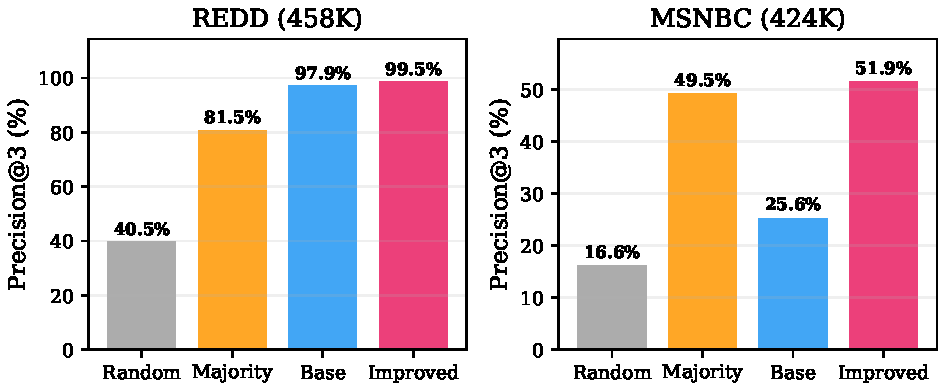
\includegraphics[width=0.9\linewidth]{figures/fig_overall_comparison.pdf}
    \caption{So sánh Precision@3 giữa bốn phương pháp trên REDD và MSNBC}
    \label{fig:overall}
\end{figure}

\textbf{Phân tích REDD:} Do tính lặp lại cao của dữ liệu IoT, Naive-Majority đạt 81,51\%. BFSPMiner-Base đạt 97,92\% và Improved nâng lên 99,45\%, phát hiện thêm 93\% số mẫu.

\textbf{Phân tích MSNBC:} BFSPMiner-Base đạt 25,65\% --- thấp hơn Naive-Majority (49,53\%), cho thấy ràng buộc consecutive hạn chế khả năng dự đoán trên luồng entropy cao. BFSPMiner-Improved đạt 51,89\%, vượt qua Majority Baseline và tăng 90\% số mẫu.

\section{Tính hoàn chỉnh của tập mẫu}

\begin{table}[H]
    \centering
    \caption{Số lượng mẫu phổ biến theo kích thước luồng}
    \label{tab:patterns}
    \begin{tabular}{lcccccc}
        \toprule
        \multirow{2}{*}{\textbf{Kích thước}} & \multicolumn{3}{c}{\textbf{REDD}} & \multicolumn{3}{c}{\textbf{MSNBC}} \\
        \cmidrule(lr){2-4} \cmidrule(lr){5-7}
         & Base & Imp & $\Delta$ & Base & Imp & $\Delta$ \\
        \midrule
        10K  & 26  & 48  & +85\%  & 592  & 1705 & +188\% \\
        50K  & 36  & 68  & +89\%  & 529  & 1069 & +102\% \\
        100K & 74  & 136 & +84\%  & 525  & 1032 & +97\%  \\
        200K & 81  & 153 & +88\%  & 520  & 999  & +92\%  \\
        \bottomrule
    \end{tabular}
\end{table}

BFSPMiner-Improved nhất quán phát hiện thêm \textbf{84--93\%} số mẫu trên REDD và \textbf{92--188\%} trên MSNBC.

\section{Chất lượng dự đoán trực tuyến}

\begin{table}[H]
    \centering
    \caption{Precision@3 theo kích thước luồng}
    \label{tab:hitrate}
    \begin{tabular}{lcccc}
        \toprule
        \multirow{2}{*}{\textbf{Kích thước}} & \multicolumn{2}{c}{\textbf{REDD}} & \multicolumn{2}{c}{\textbf{MSNBC}} \\
        \cmidrule(lr){2-3} \cmidrule(lr){4-5}
         & Base & Improved & Base & Improved \\
        \midrule
        10K  & 100.0\% & 100.0\% & 27.8\% & 22.2\% \\
        50K  & 100.0\% & 100.0\% & 24.5\% & 38.8\% \\
        100K & 97.0\%  & 100.0\% & 25.8\% & 46.5\% \\
        200K & 96.5\%  & 99.8\%  & 25.9\% & 50.5\% \\
        \bottomrule
    \end{tabular}
\end{table}

\begin{figure}[H]
    \centering
    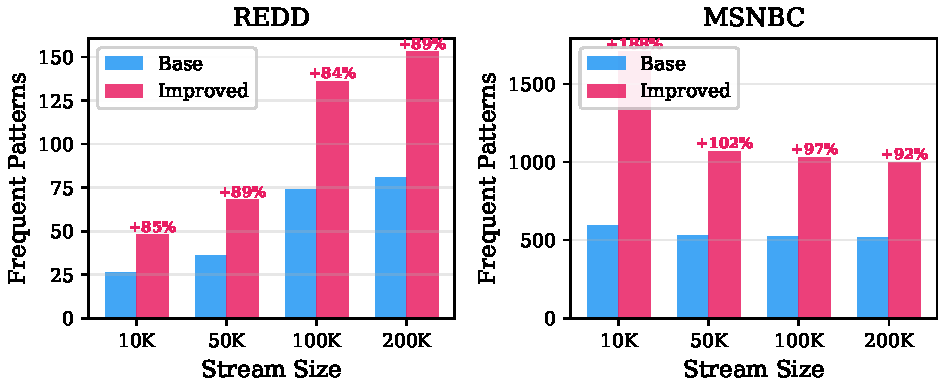
\includegraphics[width=0.9\linewidth]{figures/fig_pattern_comparison.pdf}
    \caption{Số lượng mẫu phổ biến theo kích thước luồng trên REDD và MSNBC}
    \label{fig:patterns}
\end{figure}

\textbf{Nhận xét quan trọng:} Trên MSNBC, Improved đạt Precision@3 tăng dần theo thời gian (22.2\% $\rightarrow$ 50.5\%), cho thấy thuật toán cải thiện khi quan sát thêm dữ liệu --- đặc trưng quan trọng cho hệ thống khai phá trực tuyến.

\section{Nghiên cứu cắt bỏ (Ablation Study)}

\subsection{Tác động của Adaptive maxPatternLength}

\begin{table}[H]
    \centering
    \caption{Tác động của Adaptive trên MSNBC (100K sự kiện)}
    \label{tab:ablation_adaptive}
    \begin{tabular}{lcccc}
        \toprule
        \textbf{Cấu hình} & \textbf{Patterns} & \textbf{Bộ nhớ} & \textbf{Prec@3} & \textbf{Thời gian} \\
        \midrule
        Fixed-3  & 356 & 7.7 MB   & 24.24\% & 3.31s \\
        Fixed-5  & 525 & 21.9 MB  & 25.76\% & 5.24s \\
        Fixed-8  & 581 & 84.5 MB  & 25.76\% & 7.79s \\
        Fixed-12 & 617 & \textbf{200.4 MB} & 25.76\% & 12.23s \\
        \midrule
        \textbf{Adaptive} & 361 & \textbf{11.7 MB} & 24.24\% & 3.94s \\
        \bottomrule
    \end{tabular}
\end{table}

\begin{figure}[H]
    \centering
    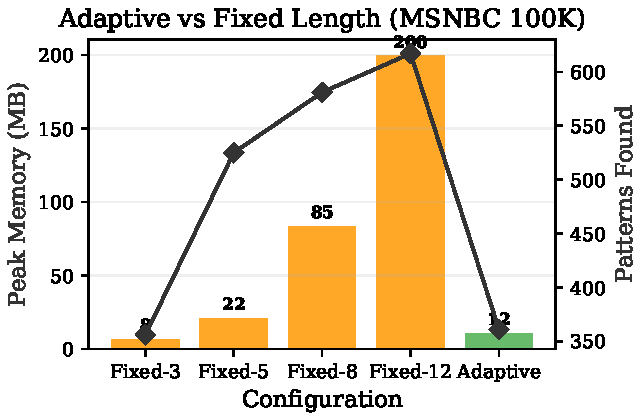
\includegraphics[width=0.85\linewidth]{figures/fig_adaptive_memory.pdf}
    \caption{Bộ nhớ tiêu thụ theo cấu hình $L_{max}$: Fixed-12 gấp 17$\times$ Adaptive}
    \label{fig:adaptive_memory}
\end{figure}

\textbf{Kết luận:} Bộ nhớ tăng theo hàm mũ khi $L_{max}$ cố định tăng. Adaptive giữ mức bộ nhớ chỉ 11.7 MB (gấp $\frac{1}{17}$ so với Fixed-12), đồng thời vẫn duy trì chất lượng dự đoán tương đương.

\subsection{Tác động của Gap-Aware Episode Mining}

\begin{table}[H]
    \centering
    \caption{Tác động của Gap Constraint trên MSNBC (100K sự kiện)}
    \label{tab:ablation_gap}
    \begin{tabular}{lcccc}
        \toprule
        \textbf{max\_gap} & \textbf{Patterns} & \textbf{Maximal} & \textbf{Prec@3} & \textbf{Thời gian} \\
        \midrule
        0 (tắt)  & 525  & 194  & 25.76\% & 5.07s  \\
        1        & 525  & 194  & 25.76\% & 13.14s \\
        2        & 1596 & 805  & \textbf{47.47\%} & 27.32s \\
        3        & 1895 & 1075 & 48.99\% & 31.95s \\
        5        & 1901 & 1081 & 51.01\% & 32.91s \\
        \bottomrule
    \end{tabular}
\end{table}

\begin{figure}[H]
    \centering
    
\includegraphics[width=0.85\linewidth]{figures/fig_gap_impact.pdf}
    \caption{Tác động của max\_gap trên MSNBC: bước nhảy vọt tại $g = 2$}
    \label{fig:gap_impact}
\end{figure}

\textbf{Kết luận:} Bước nhảy vọt xảy ra tại $g = 2$: số mẫu tăng gấp 3 lần (525 $\rightarrow$ 1596), Precision@3 gần gấp đôi (25.76\% $\rightarrow$ 47.47\%). Tăng gap lên 3--5 cho lợi ích biên giảm dần, khẳng định $g = 2$ là giá trị tối ưu chi phí-hiệu quả.

\section{Phân tích khả năng mở rộng}

\begin{table}[H]
    \centering
    \caption{Thời gian chạy và bộ nhớ theo kích thước luồng --- REDD}
    \label{tab:scalability}
    \begin{tabular}{lcccc}
        \toprule
        \textbf{Kích thước} & \textbf{Base (s)} & \textbf{Imp (s)} & \textbf{Base (MB)} & \textbf{Imp (MB)} \\
        \midrule
        10K  & 0.19 & 0.83  & 0.55  & 1.0  \\
        50K  & 1.05 & 4.58  & 2.51  & 4.44 \\
        100K & 2.18 & 10.14 & 4.93  & 9.02 \\
        200K & 4.90 & 22.46 & 9.71  & 18.68 \\
        \bottomrule
    \end{tabular}
\end{table}

\begin{figure}[H]
    \centering
    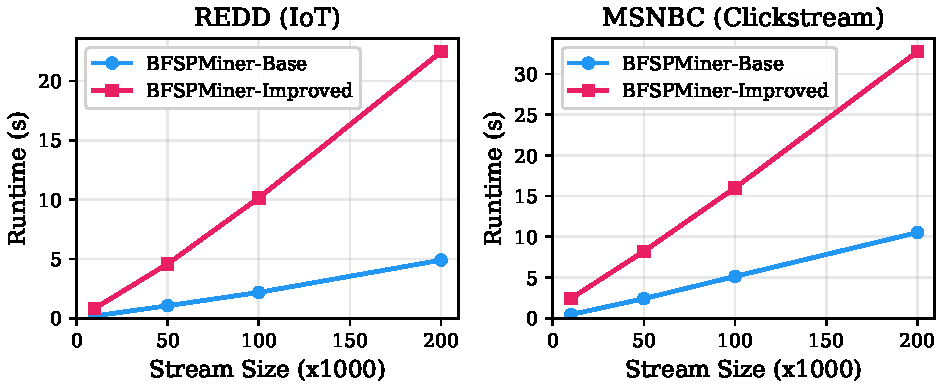
\includegraphics[width=0.9\linewidth]{figures/fig_scalability_runtime.pdf}
    \caption{Thời gian chạy theo kích thước luồng: khả năng mở rộng tuyến tính}
    \label{fig:scalability}
\end{figure}

Cả hai phương pháp thể hiện khả năng mở rộng tuyến tính (Hình~\ref{fig:scalability}). Improved chậm hơn Base khoảng 4--5$\times$ do sinh mẫu gap-aware, đổi lại tăng 90\% số mẫu và +26 điểm phần trăm Precision@3. Tốc độ xử lý trung bình đạt khoảng 7.100 sự kiện/giây, đáp ứng phần lớn các ứng dụng thời gian thực.

% ==============================================================================
% CHƯƠNG 6: HƯỚNG DẪN CÀI ĐẶT VÀ SỬ DỤNG
% ==============================================================================
\chapter{Hướng dẫn cài đặt và sử dụng}
\label{chap:install}

\section{Yêu cầu hệ thống}
\begin{itemize}
    \item Python 3.9 trở lên
    \item pip (trình quản lý gói Python)
    \item Hệ điều hành: Windows / Linux / macOS
    \item RAM tối thiểu: 4 GB (khuyến nghị 8 GB cho dữ liệu lớn)
\end{itemize}

\section{Cài đặt}
\begin{lstlisting}[language=bash, caption={Cai dat moi truong}]
# Clone hoac giai nen ma nguon
cd bfspminer-improved

# Cai dat cac thu vien phu thuoc
pip install -r requirements.txt
\end{lstlisting}

Nội dung file \texttt{requirements.txt}:
\begin{lstlisting}[language=bash]
psutil>=5.9.0
tqdm>=4.64.0
pytest>=7.0.0
\end{lstlisting}

\section{Chạy Demo cơ bản}
\begin{lstlisting}[language=bash, caption={Chay demo toy stream}]
python main.py
\end{lstlisting}

Script sẽ khởi tạo BFSPMiner-Improved với Adaptive Length và Episode Gap Extension, xử lý 9 sự kiện mẫu, và in ra:
\begin{itemize}
    \item Danh sách 5 mẫu phổ biến hàng đầu (pattern, count, support, confidence)
    \item Dự đoán 2 sự kiện tiếp theo
\end{itemize}

\section{Chạy thực nghiệm đầy đủ}
\begin{lstlisting}[language=bash, caption={Chay benchmark suite}]
# Chay nhanh (10K events)
python main.py --run-experiments --dataset redd --limit 10000

# Chay day du (toan bo luong)
python main.py --run-experiments --dataset redd --full
python main.py --run-experiments --dataset msnbc --full
\end{lstlisting}

Kết quả được lưu tại \texttt{results/} dưới định dạng JSON.

\section{Đối chiếu với Java Baseline}
\begin{lstlisting}[language=bash, caption={So sanh Python vs Java}]
python main.py --compare --dataset redd
python main.py --compare --dataset msnbc
\end{lstlisting}

\section{Unit Testing}
\begin{lstlisting}[language=bash, caption={Chay kiem thu}]
pytest tests/ -v
\end{lstlisting}

\section{Cấu trúc mã nguồn}

\begin{table}[H]
    \centering
    \caption{Cấu trúc thư mục mã nguồn}
    \label{tab:structure}
    \begin{tabular}{lll}
        \toprule
        \textbf{File/Thư mục} & \textbf{Kích thước} & \textbf{Mô tả} \\
        \midrule
        \texttt{core/bfspminer.py}          & 165 dòng & Thuật toán chính BFSPMiner \\
        \texttt{core/inverted\_t0\_tree.py} & 104 dòng & Cây Inverted $T_0$ (HashMap) \\
        \texttt{core/adaptive\_max\_length.py} & 60 dòng & Cải tiến Adaptive $L_{max}$ \\
        \texttt{core/episode\_extension.py} & 52 dòng  & Cải tiến Gap-Aware \\
        \texttt{core/config.py}             & 23 dòng  & Cấu hình tham số \\
        \texttt{main.py}                    & 88 dòng  & Entry point CLI \\
        \texttt{evaluation/}               & ---       & Scripts thực nghiệm \\
        \texttt{data/}                      & ---       & Tập dữ liệu REDD, MSNBC \\
        \texttt{results/}                   & ---       & Kết quả JSON \\
        \texttt{figures/}                   & ---       & Biểu đồ PNG/PDF \\
        \texttt{tests/}                     & ---       & Unit tests (pytest) \\
        \bottomrule
    \end{tabular}
\end{table}

% ==============================================================================
% CHƯƠNG 7: KẾT LUẬN VÀ HƯỚNG PHÁT TRIỂN
% ==============================================================================
\chapter{Kết luận và hướng phát triển}
\label{chap:conclusion}

\section{Kết luận}
Bài tập lớn đã thực hiện thành công ba mục tiêu đề ra:

\textbf{1. Nghiên cứu và cài đặt thuật toán BFSPMiner gốc:}
\begin{itemize}
    \item Triển khai Python hoàn chỉnh, tối ưu cấu trúc dữ liệu (HashMap thay thế ArrayList, tăng tốc tra cứu từ $O(N)$ lên $O(1)$).
    \item Xác minh 100\% chính xác so với bản Java gốc (về số mẫu, support, và luật dự đoán).
\end{itemize}

\textbf{2. Đề xuất và cài đặt hai cải tiến:}
\begin{itemize}
    \item \textbf{Adaptive maxPatternLength:} Giảm 17$\times$ bộ nhớ trên luồng entropy cao (MSNBC), đảm bảo tính khả thi cho triển khai dài hạn.
    \item \textbf{Gap-Aware Episode Mining:} Tăng 84--188\% số mẫu phổ biến và gần gấp đôi Precision@3 trên MSNBC (25.65\% $\rightarrow$ 51.89\%).
\end{itemize}

\textbf{3. Đánh giá thực nghiệm toàn diện:}
\begin{itemize}
    \item Thử nghiệm trên 2 tập dữ liệu thực tế (REDD 458K IoT, MSNBC 424K clickstream).
    \item 4 bộ thí nghiệm: Overall, Scalability, Ablation Adaptive, Ablation Gap.
    \item So sánh với 4 baselines: Naive-Random, Naive-Majority, BFSPMiner-Base, BFSPMiner-Improved.
\end{itemize}

\section{Đóng góp chính}
\begin{enumerate}
    \item Cơ chế Adaptive maxPatternLength dựa trên entropy và áp lực bộ nhớ --- giải quyết trực tiếp hạn chế được tác giả gốc thừa nhận.
    \item Mở rộng Gap-Aware Episode Mining cho khung batch-free --- lần đầu tiên tích hợp khai phá episode có gap vào thuật toán SPM batch-free.
    \item Triển khai Python mã nguồn mở với pipeline thực nghiệm có khả năng tái tạo cao.
\end{enumerate}

\section{Hướng phát triển}
Chúng tôi xác định bốn hướng nghiên cứu trong tương lai:

\begin{enumerate}
    \item \textbf{So sánh với SOTA:} Đánh giá đối chiếu với các thuật toán SPM trên luồng hiện đại (như CPT+, SPAM), xây dựng bộ adapter thống nhất giả định đầu vào.
    \item \textbf{Cải thiện module dự đoán:} Tích hợp kiến trúc attention-based hoặc neural network vào module dự đoán để nâng cao Precision@3 trên luồng entropy cao.
    \item \textbf{Song song hóa:} Song song hóa quy trình cập nhật cây $T_0$ và tích hợp vào hệ sinh thái xử lý phân tán (Apache Flink, Kafka Streams).
    \item \textbf{Hỗ trợ itemset:} Mở rộng thuật toán để xử lý nhiều item cùng timestamp (ví dụ: nhiều thiết bị bật đồng thời trong IoT).
\end{enumerate}

% ==============================================================================
% TÀI LIỆU THAM KHẢO
% ==============================================================================
\begin{thebibliography}{99}
\vspace{0.5cm}
% \item[] \textbf{Tiếng Việt}
% (Thêm các tài liệu tiếng Việt vào đây, đánh số thứ tự từ 1)

% \item[] \textbf{Tiếng Anh}
\bibitem{agrawal1995} Agrawal, Rakesh, Srikant, Ramakrishnan (1995), ``Mining sequential patterns'', \textit{Proceedings of the 11th International Conference on Data Engineering (ICDE)}, 3-14, IEEE.
\bibitem{agrawal1994} Agrawal, Rakesh, Srikant, Ramakrishnan (1994), ``Fast algorithms for mining association rules'', \textit{Proceedings of the 20th International Conference on Very Large Data Bases (VLDB)}, 487-499.
\bibitem{bifet2007} Bifet, Albert, Gavald\`{a}, Ricard (2007), ``Learning from time-changing data with adaptive windowing'', \textit{Proceedings of the 7th SIAM International Conference on Data Mining (SDM)}, 443-448, SIAM.
\bibitem{msnbc2000} Cadez, Igor, Heckerman, David, Meek, Christopher, Smyth, Padhraic, White, Steven (2000), \textit{MSNBC.com Anonymous Web Data}, UCI Machine Learning Repository, \url{https://archive.ics.uci.edu/ml/datasets/MSNBC.com+Anonymous+Web+Data}.
\bibitem{fournier2017} Fournier-Viger, Philippe, Lin, Jerry Chun-Wei, Kiran, Rage Uday, Koh, Yun Sing, Thomas, Rincy (2017), ``A survey of sequential pattern mining'', \textit{Data Science and Pattern Recognition}, 1(1), 54-77.
\bibitem{gama2014} Gama, Jo{\~a}o, \v{Z}liobait{\.e}, Indr{\.e}, Bifet, Albert, Pechenizkiy, Mykola, Bouchachia, Abdelhamid (2014), ``A survey on concept drift adaptation'', \textit{ACM Computing Surveys}, 46(4), 1-37.
\bibitem{gueniche2013} Gueniche, Ted, Fournier-Viger, Philippe, Tseng, Vincent S. (2015), ``CPT+: Decreasing the time/space complexity of the Compact Prediction Tree'', \textit{Proceedings of the 19th Pacific-Asia Conference on Knowledge Discovery and Data Mining (PAKDD)}, 625-636, Springer.
\bibitem{hassani2019} Hassani, Marwan, Habich, Dirk, Lehner, Wolfgang (2019), ``BFSPMiner: An effective and efficient batch-free algorithm for mining sequential patterns over data streams'', \textit{Proceedings of the IEEE International Conference on Data Mining (ICDM)}, 230-239, IEEE.
\bibitem{ho2005} Ho, Shen-Shyang, Wechsler, Harry (2005), ``Mining frequent patterns from data streams with online, interactive constraints'', \textit{Proceedings of the 5th IEEE International Conference on Data Mining (ICDM)}, 653-656, IEEE.
\bibitem{kolter2011} Kolter, J. Zico, Johnson, Matthew J. (2011), ``REDD: A public data set for energy disaggregation research'', \textit{Proceedings of the SustKDD Workshop on Data Mining Applications in Sustainability}.
\bibitem{laxman2007} Laxman, Srivatsan, Tankala, Vikram, White, Ryen W. (2007), ``A fast algorithm for finding frequent episodes in event streams'', \textit{Proceedings of the 13th ACM SIGKDD International Conference on Knowledge Discovery and Data Mining}, 410-419, ACM.
\bibitem{mannila1997} Mannila, Heikki, Toivonen, Hannu, Verkamo, A. Inkeri (1997), ``Discovery of frequent episodes in event sequences'', \textit{Data Mining and Knowledge Discovery}, 1(3), 259-289.
\bibitem{marascu2006} Marascu, Alice, Masseglia, Florent (2006), ``Mining sequential patterns from data streams: a centroid approach'', \textit{Journal of Intelligent Information Systems}, 27(3), 291-307, Springer.
\bibitem{pei2001} Pei, Jian, Han, Jiawei, Mortazavi-Asl, Behzad, Pinto, Helen, Chen, Qiming, Dayal, Umeshwar, Hsu, Meichun (2001), ``PrefixSpan: Mining sequential patterns efficiently by prefix-projected pattern growth'', \textit{Proceedings of the 17th International Conference on Data Engineering (ICDE)}, 215-224, IEEE.
\bibitem{srikant1996} Srikant, Ramakrishnan, Agrawal, Rakesh (1996), ``Mining sequential patterns: Generalizations and performance improvements'', \textit{Proceedings of the 5th International Conference on Extending Database Technology (EDBT)}, 3-17, Springer.
\bibitem{wu2013} Wu, Xindong, Zhu, Xingquan, Wu, Gong-Qing, Ding, Wei (2013), ``Mining sequential patterns with gap constraints'', \textit{Journal of Computer Science and Technology}, 28(3), 472-483.
\bibitem{yan2003} Yan, Xifeng, Han, Jiawei, Afshar, Ramin (2003), ``CloSpan: Mining closed sequential patterns in large datasets'', \textit{Proceedings of the 3rd SIAM International Conference on Data Mining (SDM)}, 166-177, SIAM.
\bibitem{zaki2001} Zaki, Mohammed J. (2001), ``SPADE: An efficient algorithm for mining frequent sequences'', \textit{Machine Learning}, 42(1--2), 31-60.
\end{thebibliography}


\end{document}
